% Copyright (C) 2013 Columbia University in the City of New York and others.
%
% Please see the AUTHORS file in the main source directory for a full list
% of contributors.
%
% This file is part of TerraFERMA.
%
% TerraFERMA is free software: you can redistribute it and/or modify
% it under the terms of the GNU Lesser General Public License as published by
% the Free Software Foundation, either version 3 of the License, or
% (at your option) any later version.
%
% TerraFERMA is distributed in the hope that it will be useful,
% but WITHOUT ANY WARRANTY; without even the implied warranty of
% MERCHANTABILITY or FITNESS FOR A PARTICULAR PURPOSE. See the
% GNU Lesser General Public License for more details.
%
% You should have received a copy of the GNU Lesser General Public License
% along with TerraFERMA. If not, see <http://www.gnu.org/licenses/>.

\usepackage[english]{babel}
%\usepackage{tgtermes}
\usepackage[colorlinks=true]{hyperref}

\usepackage{mathpazo}
\usepackage[protrusion=true,expansion=true]{microtype}
\usepackage{lettrine}
\usepackage{graphicx}
\usepackage{amsfonts,amsmath,amssymb,amsthm,amsbsy,amssymb,bm}
\usepackage{xcolor}
\usepackage{enumitem}

\usepackage[square,sort,comma,numbers]{natbib}
\usepackage{rotating}
\setlength\fboxrule{0.0pt}
\setlength\fboxsep{0pt}

% Units
\usepackage{units}

\newcommand{\m}[1][]{\unit[#1]{m}}
\newcommand{\mm}[1][]{\unit[#1]{mm}}
\newcommand{\km}[1][]{\unit[#1]{km}}
\newcommand{\s}[1][]{\unit[#1]{s}}
\newcommand{\hrs}[1][]{\unit[#1]{hrs}}
\newcommand{\invs}[1][]{\unit[#1]{s}\ensuremath{^{-1}}}
\newcommand{\ms}[1][]{\unit[#1]{m\ensuremath{\,}s\ensuremath{^{-1}}}}
\newcommand{\mss}[1][]{\unit[#1]{m\ensuremath{\,}s\ensuremath{^{-2}}}}
\newcommand{\J}[1][]{\unit[#1]{J}}
\newcommand{\K}[1][]{\unit[#1]{K}}
\newcommand{\W}[1][]{\unit[#1]{W}}
\newcommand{\PSU}[1][]{\unit[#1]{PSU}}
\newcommand{\Pa}[1][]{\unit[#1]{Pa}}
\newcommand{\kg}[1][]{\unit[#1]{kg}}
\newcommand{\rads}[1][]{\unit[#1]{rad\ensuremath{\,}s\ensuremath{^{-1}}}}
\newcommand{\kgmm}[1][]{\unit[#1]{kg\ensuremath{\,}m\ensuremath{^{-2}}}}
\newcommand{\kgmmm}[1][]{\unit[#1]{kg\ensuremath{\,}m\ensuremath{^{-3}}}}
\newcommand{\Nmm}[1][]{\unit[#1]{N\ensuremath{\,}m\ensuremath{^{-2}}}}
\newcommand\Celsius{\ensuremath{^\circ}\unit{C}}


\usepackage[final]{listings}
\lstloadlanguages{[LaTeX]TeX,Python,bash,[gnu]Make,XML}

\lstset{basicstyle=\footnotesize\ttfamily,
  emph=anyfield,
  emphstyle=\textit,
  morekeywords={pure},
  escapeinside=`'
}

\lstdefinestyle{Bash}{
  language=bash,
  basicstyle=\small\sffamily,
  frame=tb,
  columns=fullflexible,
  backgroundcolor=\color{yellow!20},
  linewidth=0.9\linewidth,
  xleftmargin=0.1\linewidth
}

\lstdefinestyle{UFL}{
  language=Python,
  basicstyle=\small\ttfamily,
  numbers=left,
  numberstyle=\tiny,
  numbersep=3pt,
  frame=tb,
  columns=fullflexible,
  backgroundcolor=\color{yellow!20},
  linewidth=0.9\linewidth,
  xleftmargin=0.1\linewidth
}
\lstdefinestyle{python}{
  language=Python,
  basicstyle=\small\sffamily,
  numbers=left,
  numberstyle=\tiny,
  numbersep=3pt,
  frame=tb,
  columns=fullflexible,
  backgroundcolor=\color{yellow!20},
  linewidth=0.9\linewidth,
  xleftmargin=0.1\linewidth
}

%%%%%%%%%%%%tikz stuff
\usepackage{tikz}
\tikzstyle{every picture}+=[remember picture]

\tikzset{onslide/.code args={<#1>#2}{%
  \only<#1>{\pgfkeysalso{#2}} % \pgfkeysalso doesn't change the path
}}
\tikzstyle{highlightred}=[shape=rectangle, rounded corners, fill=red!50]
\tikzstyle{highlightgreen}=[shape=rectangle, rounded corners, fill=green!50]

\usetikzlibrary{fit, positioning, trees}
\usetikzlibrary{decorations.markings}
\usetikzlibrary{arrows,shapes}
\tikzstyle arrowstyle=[scale=1]
\tikzset{%
  highlight/.style={rectangle,rounded corners,fill opacity=0.5,inner sep=0pt}
}
\newcommand{\tikzmark}[2]{\tikz[overlay,remember picture,baseline=(#1.base)] \node (#1) {#2};}
%
\newcommand{\tikzhighlight}[4]{%
    \tikz[overlay,remember picture]{
    \node[highlight,fill=#4,fit=(#2.north west) (#3.south east)] (#1) {};}
}

\newcommand{\tikztermhighlight}[3]{\tikz[baseline=(#2.base)] \node[onslide=<#1>{highlightred}] (#2) {#3};}
\newcommand{\tikztermhighlightgreen}[3]{\tikz[baseline=(#2.base)] \node[onslide=<#1>{highlightgreen}] (#2) {#3};}

\tikzset{hide on/.code={\only<#1>{\pgfkeysalso{opacity=0}}}}

\tikzstyle directed=[postaction={decorate,decoration={markings,
    mark=at position 1.0 with {\arrow[arrowstyle]{stealth}}}}]
\tikzstyle reverse directed=[postaction={decorate,decoration={markings,
    mark=at position .65 with
    {\arrowreversed[arrowstyle]{stealth};}}}]
%%%%%%%%%%%%%%%%%%%%%%%%%%%%%
\usepackage{macros}
\addtolength{\textwidth}{2cm}
\addtolength{\foremargin}{-2cm}
\checkandfixthelayout

% See the ``Memoir customise'' template for some common customisations
% Don't forget to read the Memoir manual: memman.pdf

% \title{A Tutorial Cookbook for \TF{}}
% \author{Marc Spiegelman and Cian Wilson\\
% Columbia University/Lamont Doherty Earth Obs.}
% \date{} % Delete this line to display the current date

%% BEGIN TITLE

\makeatletter
\def\maketitle{%
  \null
  \thispagestyle{empty}%
  \vfill
  \begin{center}\leavevmode
    \normalfont
    {\LARGE\raggedleft \@author\par}%
    \hrulefill\par
    {\huge\raggedright \@title\par}%
    %\vskip 1cm
    %\vfill
    \vskip 1cm
    %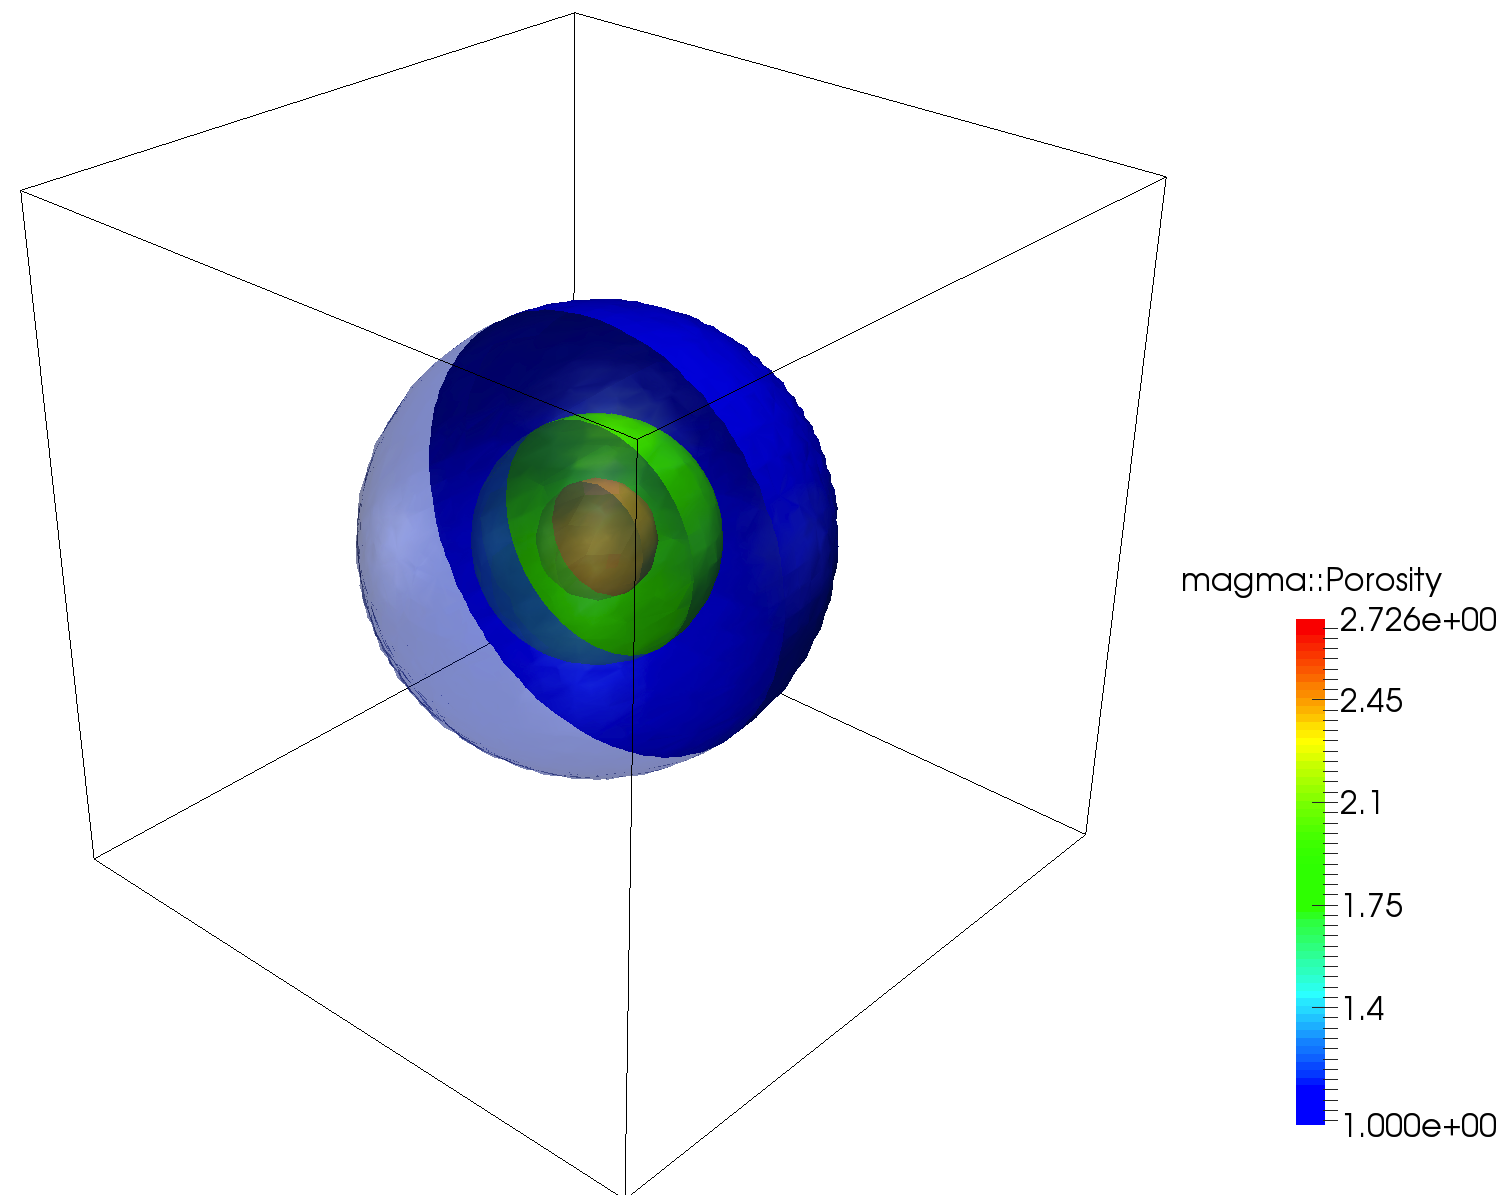
\includegraphics[width=.9\textwidth]{figures/3D_Solitary_Wave_c5n3m0b_cropped.png}\\
    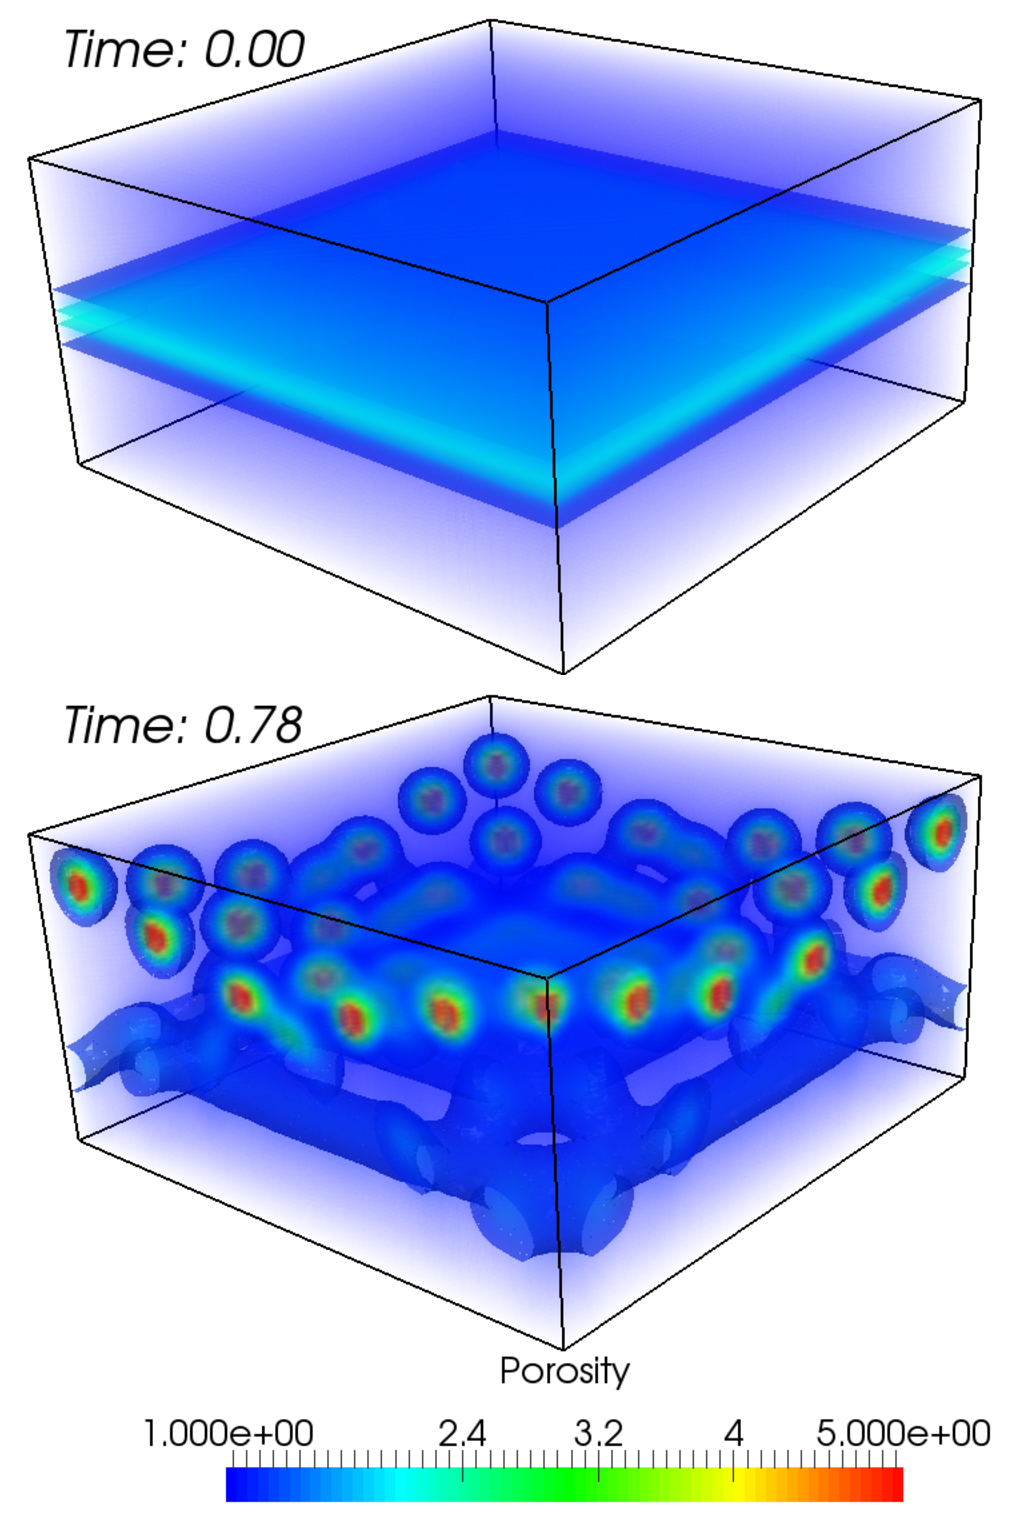
\includegraphics[width=.65\textwidth]{figures/1dto3dwaves.pdf}\\
    %\vfill{}
    \vskip 0.5cm
    {\Large Version 1.0\par}%
    {\Large \@date\par}%
  \end{center}%
  \vfill
  \null
  \cleardoublepage
  }
\makeatother
\author{Marc Spiegelman and Cian Wilson}
\title{A Tutorial Cookbook for \TF{}}
\date{\today}

%%% HEADERS & FOOTERS
\pagestyle{ruled} % try also: empty , plain , headings , ruled , Ruled , companion

%%% CHAPTERS
\chapterstyle{demo} % try also: default , section , hangnum , companion , article, demo

%%% Change section number depth
\setsecnumdepth{subsection}
\setcounter{tocdepth}{2}

%%% clean up bib with Siam.bst \sc{} is not supported for some reason
\renewcommand{\sc}{}





